\section{Modeling of Giraf administration}
To be able to view the Giraf administration system as a model, a class diagram was made, see figure \vref{fig:classOversigt}. This gives an overview of what we have to implement in our program and the class diagram describes how the base model would look like. Before the Giraf administration system gets requested applications to administer, the system needs a user. In the model there are three different individuals, the child and the users of the system, either a parent or a kindergarten teacher. To detect which Giraf mobile applications a child's device has, a user must have a connection to the child. The difference between the Giraf administration system and the administration application is that the application has access to settings for each application on the device e.g. DigiPECS or aSchedule, whereas all applications, their settings and the device's settings are all accessible from the Giraf administration system.
\pagebreak

\begin{figure}[!ht]
	\centering
		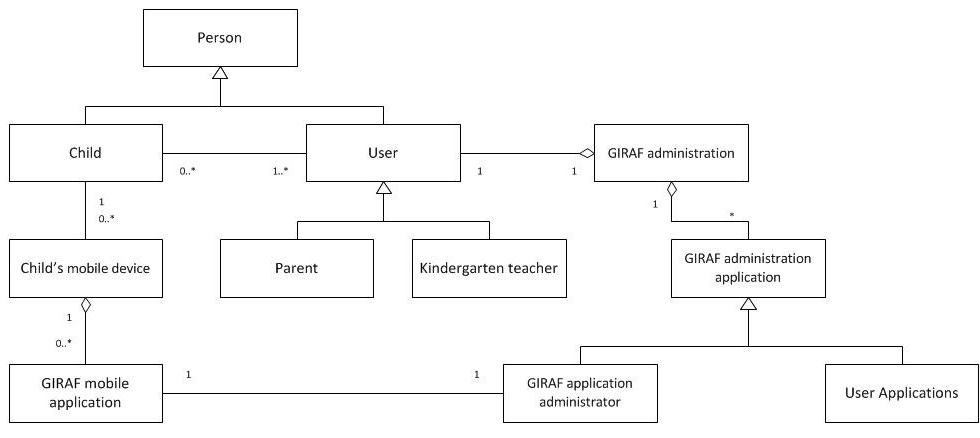
\includegraphics[width=1.00\textwidth]{img/classOversigt.jpg}
	\caption{Giraf administration program}
	\label{fig:classOversigt}
\end{figure}
